% Autor: Leonhard Segger, Alexander Neuwirth
% Datum: 2017-10-30
\documentclass[
	% Papierformat
	a4paper,
	% Schriftgröße (beliebige Größen mit „fontsize=Xpt“)
	12pt,
	% Schreibt die Papiergröße korrekt ins Ausgabedokument
	pagesize,
	% Sprache für z.B. Babel
	ngerman
]{scrartcl}

% Achtung: Die Reihenfolge der Pakete kann (leider) wichtig sein!
% Insbesondere sollten (so wie hier) babel, fontenc und inputenc (in dieser
% Reihenfolge) als Erstes und hyperref und cleveref (Reihenfolge auch hier
% beachten) als Letztes geladen werden!

\usepackage{tikz}
\usetikzlibrary{calc,patterns,angles,quotes} % loads some tikz extensions\usepackage{tikz}
\usetikzlibrary{babel}

% Silbentrennung etc.; Sprache wird durch Option bei \documentclass festgelegt
\usepackage{babel}
% Verwendung der Zeichentabelle T1 (Sonderzeichen etc.)
\usepackage[T1]{fontenc}
% Legt die Zeichenkodierung der Eingabedatei fest, z.B. UTF-8
\usepackage[utf8]{inputenc}
% Schriftart
\usepackage{lmodern}
% Zusätzliche Sonderzeichen
\usepackage{textcomp}

% Mathepaket (intlimits: Grenzen über/unter Integralzeichen)
\usepackage[intlimits]{amsmath}
% Ermöglicht die Nutzung von \SI{Zahl}{Einheit} u.a.
\usepackage{siunitx}
% Zum flexiblen Einbinden von Grafiken (\includegraphics)
\usepackage{graphicx}
% Abbildungen im Fließtext
\usepackage{wrapfig}
% Abbildungen nebeneinander (subfigure, subtable)
\usepackage{subcaption}
% Funktionen für Anführungszeichen
\usepackage{csquotes}
\MakeOuterQuote{"}
% Zitieren, Bibliografie
\usepackage[sorting=none]{biblatex}


% Zur Darstellung von Webadressen
\usepackage{url}
%chemische Formeln
\usepackage[version=4]{mhchem}
% siunitx: Deutsche Ausgabe, Messfehler getrennt mit ± ausgeben
\usepackage{floatrow}
\floatsetup[table]{capposition=top}
\usepackage{float}
% Verlinkt Textstellen im PDF-Dokument
\usepackage[unicode]{hyperref}
% "Schlaue" Referenzen (nach hyperref laden!)
\usepackage{cleveref}
\sisetup{
	locale=DE,
	separate-uncertainty
}
\bibliography{BA-C-04_MI_19-11-2018_References}

\begin{document}

	\begin{titlepage}
		\centering
		{\scshape\LARGE Versuchsbericht zu \par}
		\vspace{1cm}
		{\scshape\huge MI - Michelson-Interferometer \par} %TODO fine?
		\vspace{2.5cm}
		{\LARGE Gruppe BA-C-04 \par}
		\vspace{0.5cm}

		{\large Alexander Neuwirth (E-Mail: a\_neuw01@wwu.de) \par}
		{\large Leonhard Segger (E-Mail: l\_segg03@uni-muenster.de) \par}
		\vfill

		durchgeführt am 19.11.2018\par
		betreut von\par
		{\large Victor Kärcher} %TODO Anpassen

		\vfill

		{\large \today\par}
	\end{titlepage}
	\tableofcontents
	\newpage

	%TODO mehr TODO in Default

	\section{Kurzfassung}
	% Hypothese	und deren Ergebnis, wenn Hypothese ist, dass nur Theorie erfüllt, sagen: Erwartung: Theorie aus einführung (mit reflink) erfüllt
	% Ergebnisse, auch Zahlen, mindestens wenn's halbwegs Sinn ergibt
	% Was wurde gemacht
	% manche leute wollen Passiv oder "man", manche nicht
	Das Michelson-Interferometer stellt ein mächtiges Werkzeug zur Untersuchung von Material- und Lichteigenschaften dar.
	In diesem Versuch wird es einerseits verwendet, um die Wellenlänge eines Lasers zu überprüfen, wobei festgestellt wird %TODO Vergleich Angabe gegen Messung
	Andererseits wird der Brechungsindex einer Glasplatte bestimmt, indem sie in einen Interferometerarm gebracht und rotiert wird.
	Dies ergibt einen Messwert von , was %TODO Messwert, vergleich zu Lit. Quarzglas
	Zuletzt wird die Druckabhängigkeit des Brechungsindexes von Luft und Kohlenstoffdioxid bestimmt.
	%TODO maybe Vergleich des Werts bei Atmosphärendruck


	\section{Theorie}
	%TODO allgemeines Theorie Zeugs
	\subsection{Bestimmung des Brechungsindexes von Glas durch Rotation} %TODO Titel besser
	In \cref{fig_glass_rotation} ist der Strahlengang für einen Einfallswinkel von $\alpha=0$ und $\alpha>0$ skizziert.
	Anhand derer soll nun die Formel aus der Einführung hergeleitet werden. %TODO cref und ist der Satz notwendig?
	\begin{figure}[H]
		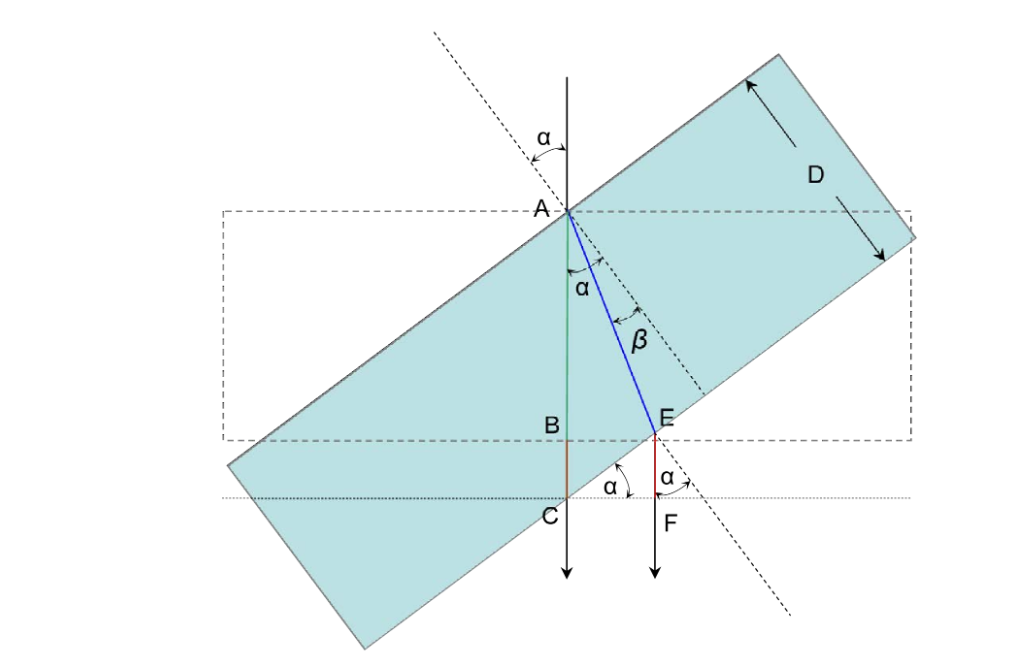
\includegraphics[width=1.0\textwidth]{images/Formula}
		\centering
		\caption{Skizze des Glas in zwei Zuständen: Einfallswinkel $\alpha= 0$ (gestrichelter Quader) und $\alpha>0$ (ausgefüllter Quader).\cite{GlasFormula}} %TODO gestrichelt fine? Quader/Quadrat %TODO cite right?
		\label{fig_glass_rotation}
		\centering
	\end{figure}

	Da sich das Glas in einem Arm des Michelson-Interferometers befindet, durchlaufen Strahlen dieses doppelt.
	Außerdem muss der Gangunterscheid $\Delta$ ein vielfaches der Wellenlänge sein. Der Gangunterschied ist die Differenz der optischen Weglängen:
	\begin{equation}
		\Delta = m\lambda = 2 \cdot \left(\int_{\text{Weg} A \rightarrow F} \! n(s) \, \mathrm{d}s - \int_{\text{Weg} A \rightarrow C} \! n(s) \, \mathrm{d}s \right)
	\end{equation}
	Aus der Geometrie und den konstanten Brechungsindizes folgt
	\begin{equation}
		m\lambda = 2(n\cdot \overline{AE} + \overline{EF} - n \cdot \overline{AB} - \overline{BC}),
		\label{eq_glas_2}
	\end{equation}
	wobei $n$ der Brechungsindex des Glas ist und $n_\text{Luft}=1$ angenommen wird.

	Unmittelbar aus \cref{fig_glass_rotation} zu entnehmen sind
		$\overline{AB} = D$,
		$\overline{AE} = \frac{D}{\cos{\beta}}$,
		$\overline{AC} = \frac{D}{\cos{\alpha}}$,
		$\overline{BC} = \overline{AC} -D = \frac{D}{\cos{\alpha}}-D$,
		$\overline{EF} = \overline{CE} \cdot \sin{\alpha} = D\cdot (\tan{\alpha}-\tan{\beta})\cdot \sin{\alpha}$.
	Ersetzt man die Strecken und dividiert durch $2D$ in \cref{eq_glas_2} folgt:
	\begin{equation}
		\frac{m\lambda}{2D} = \frac{n}{\cos{\beta}} + \sin{\alpha}\tan{\alpha} - \sin{\alpha}\tan{\beta}-n  - \frac{1}{cos{\alpha}} +1
	\end{equation}
	Durch das Snelliusssche Brechungsgesetz $n \cdot \sin{\beta} = \sin{\alpha}$  ergibt sich mit $\cos{\beta}=\sqrt{1-\frac{\sin^2{\alpha}}{n^2}}$:
	\begin{equation}
		\frac{m\lambda}{2D} = \sqrt{n^2-\sin^2{\alpha}} -\cos{\alpha} - n + 1
	\end{equation}
	und quadriert
	\begin{equation}
		\left(\frac{m\lambda}{2D}+ \cos{\alpha}-1+n\right)^2 = n^2-\sin^2{\alpha}
	\end{equation}
	Nach Ausmultiplizieren und Umformen ergibt sich:
	\begin{equation}
		n=\frac{\sin^2{\alpha}+\left(\frac{m\lambda}{2D} + \cos{\alpha}-1\right)^2}{2(1-cos{\alpha}-\frac{m\lambda}{2D})}
	\end{equation}
	Mit $\alpha=\Phi$, und $D=t$ lässt sich dies in die Formel aus der Einführung umstellen:
	\begin{equation}
		n= \frac{(2t-m\lambda)(1-\cos{\Phi})+ \frac{m^2\lambda^2}{4t}}{2t(1-\cos{\Phi})-m\lambda}
		\label{eq_brechindex}
	\end{equation}

	\section{Methoden}
	% Bilder von der Website klauen
	% einer will Präsens
	%TODO Glas Nullwinkel per Auge
	%TODO Glas Umrechnungsfaktor für Winkel
	Es soll mit dem Michelson-Interferometer die Wellenlänge eines Helium-Neon-Lasers und die Brechungsindizes von Luft, Kohlenstoffdioxid und einer Glasplatte bestimmt werden.
	Dazu wird der Aufbau in \cref{fig_aufbau} verwendet.

	\begin{figure}[H]
		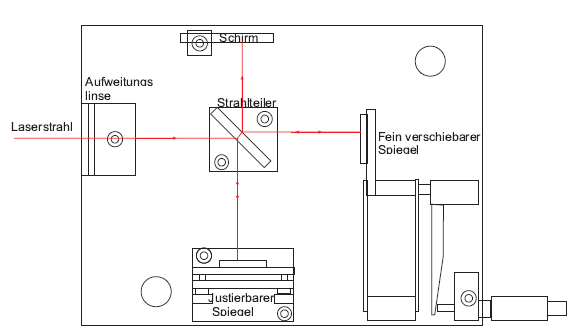
\includegraphics[width=\textwidth]{images/michelson_aufbau}
		\centering
		\caption{Aufbau des Michelson-Interferometers. \cite{Anleitung}}
		\label{fig_aufbau}
	\end{figure}
	\section{Ergebnisse und Diskussion}



	% Allgemeine Beobachtungen
	% Einflüsse von veränderten Parametern auf Messung

	% Berechung nach Aufgabenstellung
	\subsection{Bestimmung der Wellenlänge}
	\subsubsection{Beobachtung und Datenanalyse}
	Zur Bestimmung der Wellenlänge des Lasers wird der Spiegel an einem Arm des Michelson-Interferometers verschoben.
	In \cref{tb_lambda} ist die Anzahl der verschobenen Maxima und die zugehörige Verschiebung des Spiegels angegeben. %TODO besseres wording aus Methode
	Die Unsicherheit von $\Delta s$ setzt sich aus der der Mikrometerschraube $u_M=\SI{11}{nm}$ und der Genauigkeit mit welcher ein Interferenzmaximum lokalisiert wird, also dessen Breite $u_B=\SI{108}{nm}$. %TODO der Satz ist nicht verständlich %TODO schreiben was delta s ist
	Des Weiteren wird davon ausgegangen, dass man sich einmal verzählen kann.
	Es ergibt sich eine über die Messungen gemittelte Wellenlänge von \SI{650.4+-10.8}{nm}.

	\begin{table}[H]
		\centering
		\begin{tabular}{| c | c | c |}
			\hline
			  $N$ &  $\Delta s$ & $\lambda=2 \Delta s/N$\\ \hline
				25$\pm$0.3 & \SI{7905+-109}{nm} & \SI{632.4+-11.6}{nm}\\
				40$\pm$0.3& \SI{13085.1+-109}{nm} & \SI{654.3+-7.3}{nm}\\
				40$\pm$0.3& \SI{13289.7+-109}{nm} & \SI{664.5+-7.4}{nm}\\
				\hline
		\end{tabular}
		\caption{Änderung der Interferenzmaxima $N$ in Abhängigkeit von $\Delta s$ der Verschiebung des Spiegels an einem Michelson-Interferometer Arm. $\lambda$ ist die gemäß der angegeben Formel berechnete Wellenlänge. } %TODO -arm? %TODO cref für formel in theorie
		\label{tb_lambda}
	\end{table}

	\subsubsection{Diskussion}


	\subsection{Bestimmung des Brechungsindex der Glasplatte}
	\subsubsection{Beobachtung und Datenanalyse}
	Zur Bestimmung des Brechungsindex der Glasplatte lässt sich \cref{eq_brechindex} umformen:
	\begin{equation}
		(1-\cos{\phi}) = \frac{nm\lambda+\frac{m^2\lambda^2}{4t}}{m\lambda+2t(n-1)}
	\end{equation}
	Dabei ist $t= \SI{5.05+-0.05}{mm}$ die Breite der Glasplatte.
	Die Unsicherheit beim Einstellen des Winkels beträgt \SI{0.011}{\degree}.
	In \cref{fig_glas} sind die Messpunkte sowie ein Fit dargestellt.
	Der Fit liefert einen Brechungsindex von \SI{1.707+-0.013}{} für die Glasplatte für eine Wellenlänge $\lambda$ von \SI{650.4+-10.8}{nm}.

\begin{figure}[H]
		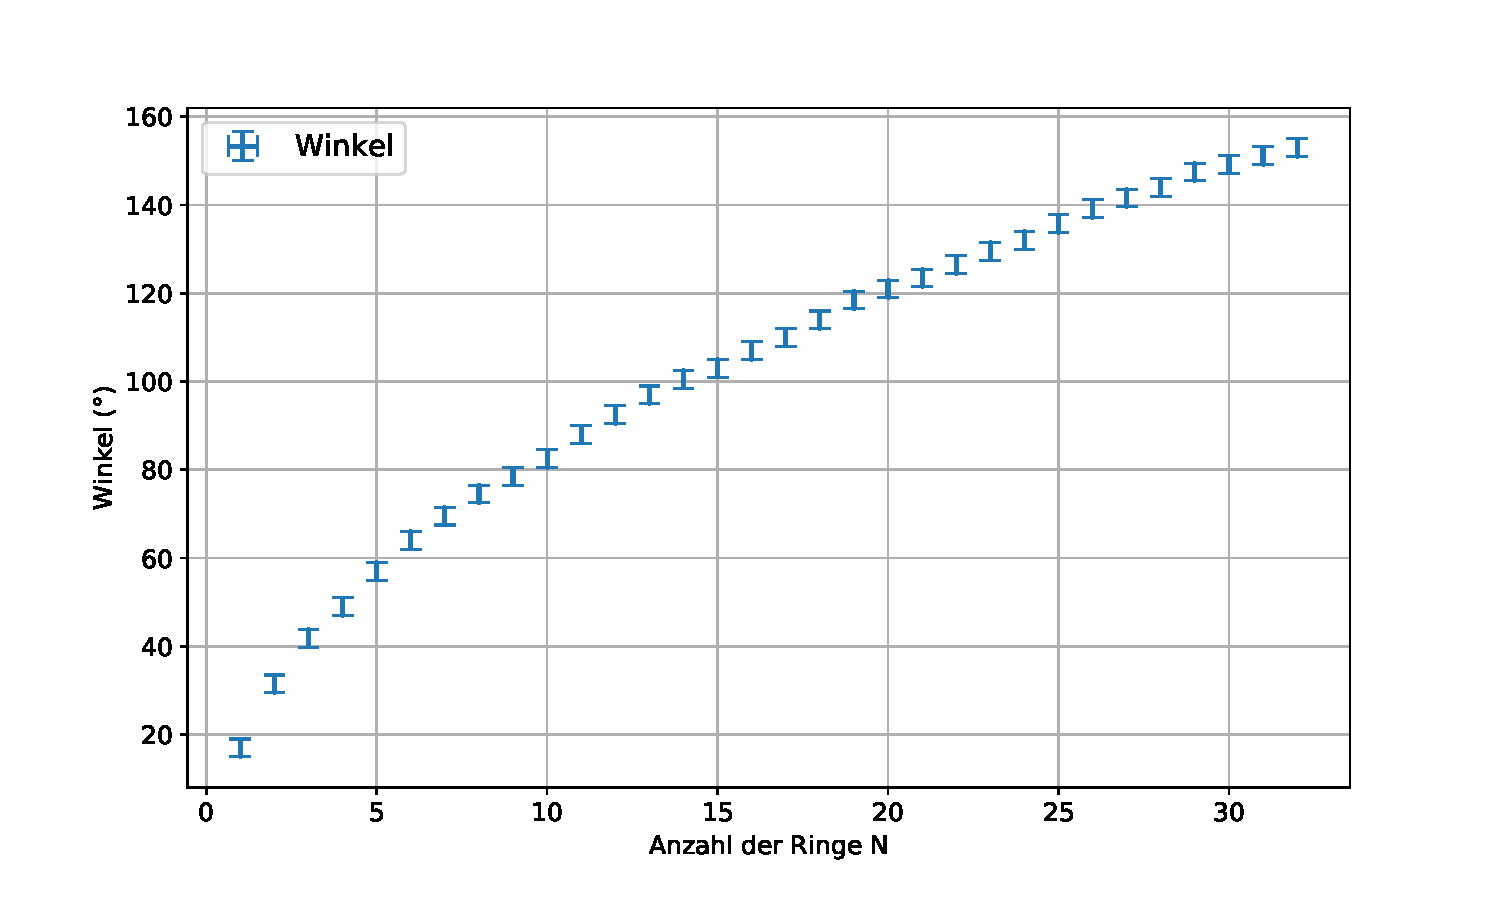
\includegraphics[width=\textwidth]{images/Glas.pdf}
		\centering
		\caption{Der Winkel der Glasplatte ist gegen die Änderung der Interferenzringe auf getragen. Die gelbe Funktion ist ein Fit gemäß den theoretischen Erwartungen.}
		\label{fig_glas}
	\end{figure}

	\subsubsection{Diskussion}

	\subsection{Bestimmung der Brechungsindizes von Gasen}
	\subsubsection{Beobachtung und Datenanalyse}
	Der Brechungsindex des jeweiligen Gases ist druckabhängig:
	\begin{equation}
		n(p) = n(p=0) + \frac{\Delta n}{\Delta p}p
	\end{equation}
	Der Brechungsindex im Vakuum $n(p=0)$ beträgt für beide Gase 1.
	Aus der Einführung ist folgender Zusammenhang bekannt: %TODO in Theorie für Ref?
	\begin{equation}
			\frac{\Delta n}{\Delta p} = \frac{\Delta m}{\Delta p} \frac{\lambda}{2l}
	\end{equation}
	Wobei $l=\SI{3.5+-0.3}{cm}$ die Länge der Küvette im Strahlengang ist, welche abgeschätzt werden musste, da die Breite des Behälters nicht bekannt ist. %TODO gucci? Breite vs Länge?
	Die Unsicherheit des Präzisions-Digital-Grobvakuummeters beträgt \SI{0.3}{mbar} und die Wellenlänge des Lasers beträgt nach wie vor \SI{650.4+-10.8}{nm}.

	In \crefrange{fig_luft_raus}{fig_co2_rein} ist der Druck $p$ gegen die Anzahl der Interferenzringe $m$ aufgetragen und es wurden lineare Fits durchgeführt, um $\Delta p / \Delta m$ und somit den Kehrwert $\Delta m / \Delta p$ zu ermitteln.


\begin{figure}[H]
		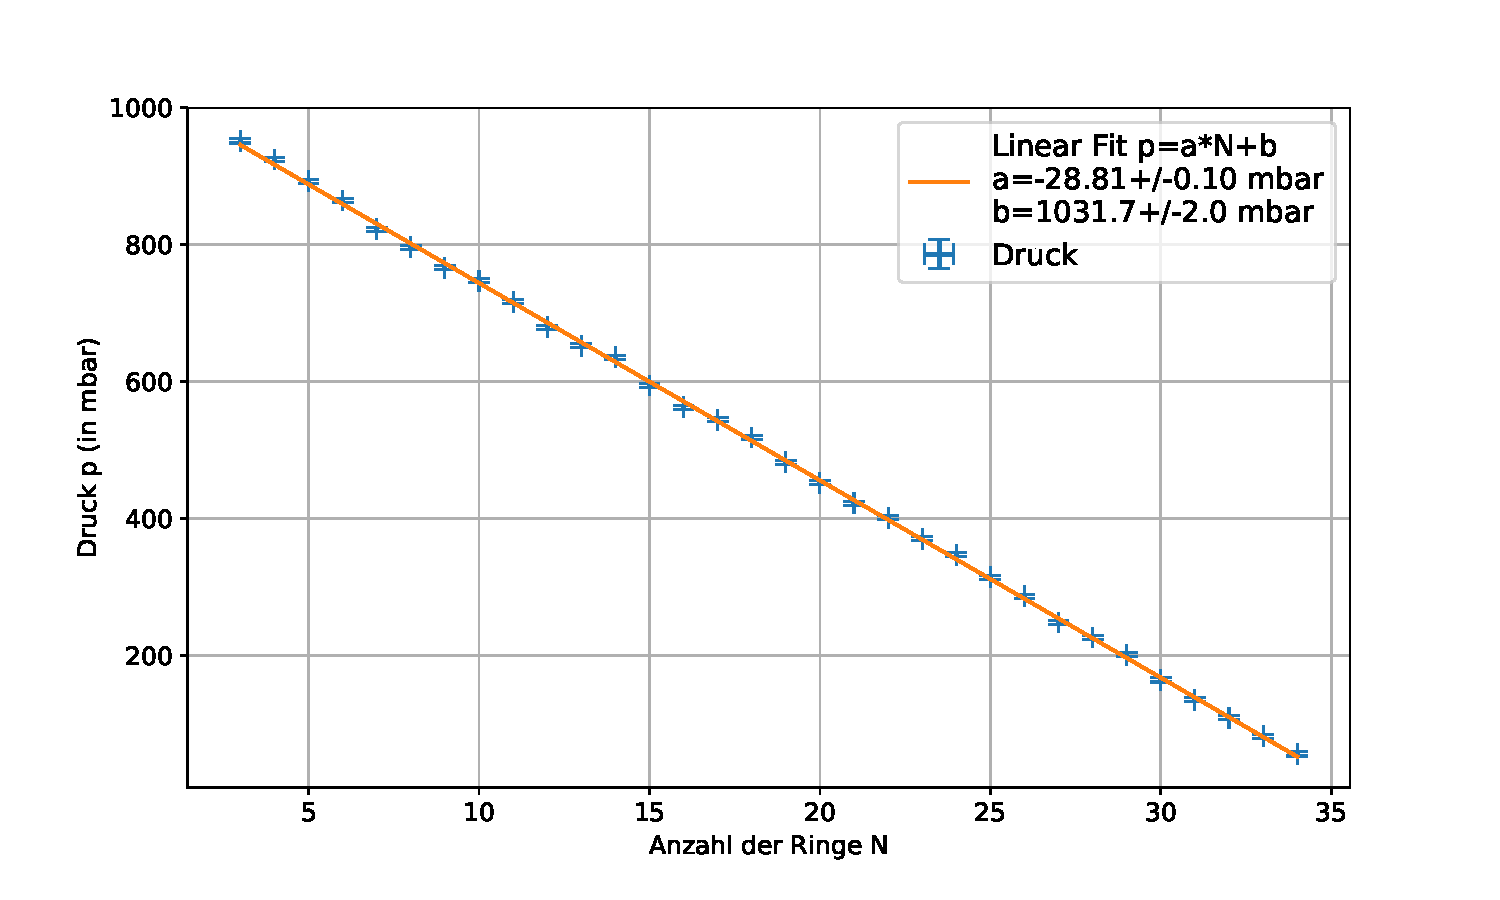
\includegraphics[width=0.9\textwidth]{images/Luft_Raus.pdf}
		\centering
		\caption{In der Küvette befindet sich Luft. Der Druck wird kontinuierlich reduziert. Die gelbe Funktion ist ein linearer Fit.}
		\label{fig_luft_raus}
	\end{figure}
\begin{figure}[H]
		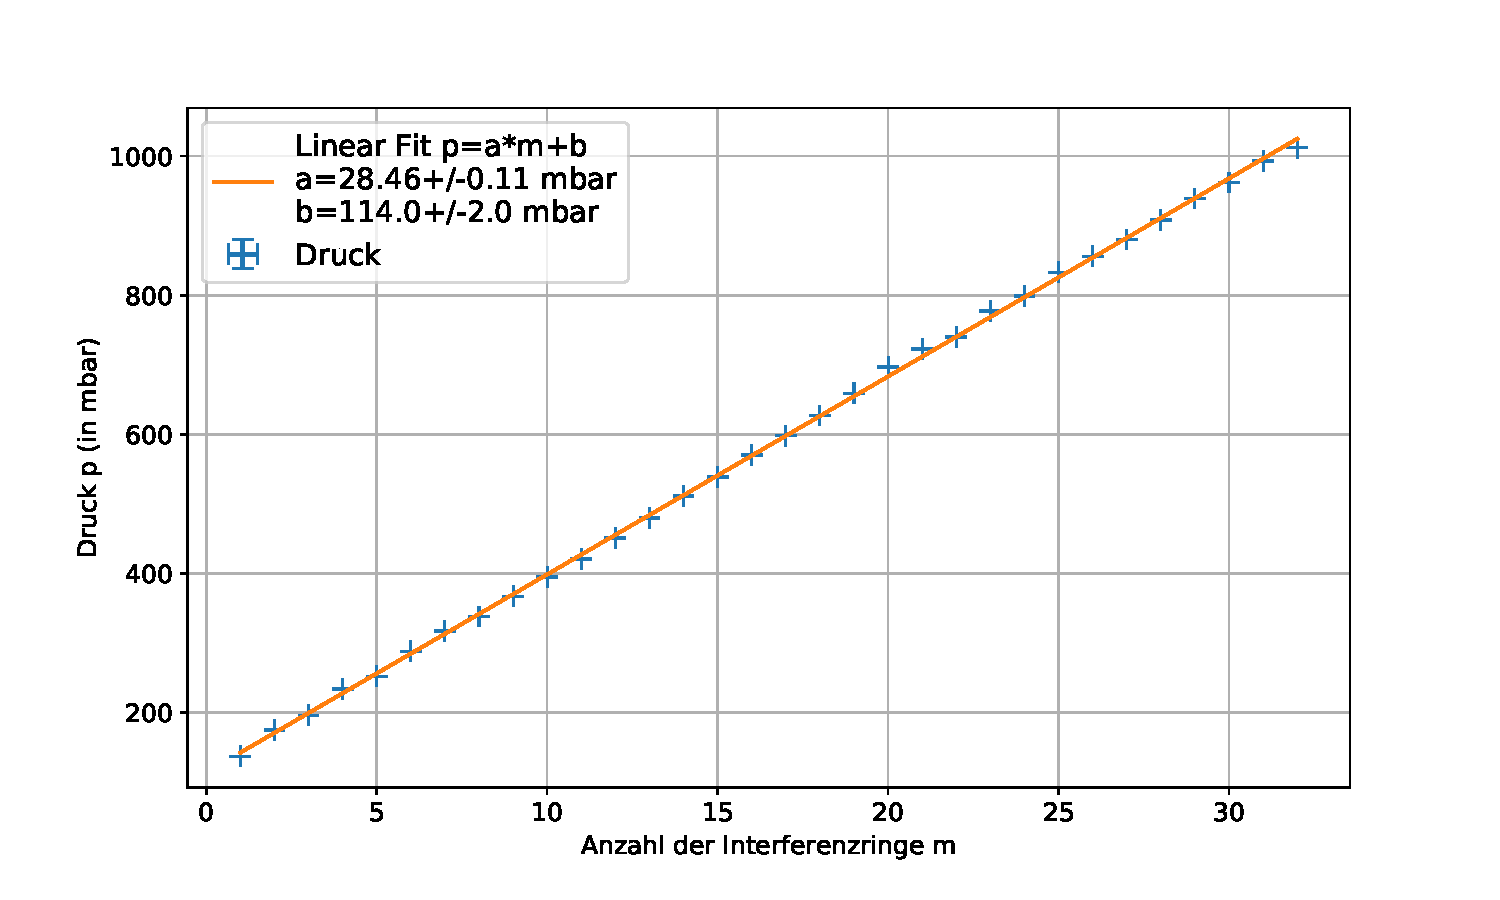
\includegraphics[width=0.9\textwidth]{images/Luft_Rein.pdf}
		\centering
		\caption{In der Küvette befindet sich Luft. Der Druck wird kontinuierlich erhöht. Die gelbe Funktion ist ein linearer Fit.}
		\label{fig_luft_rein}
	\end{figure}
\begin{figure}[H]
		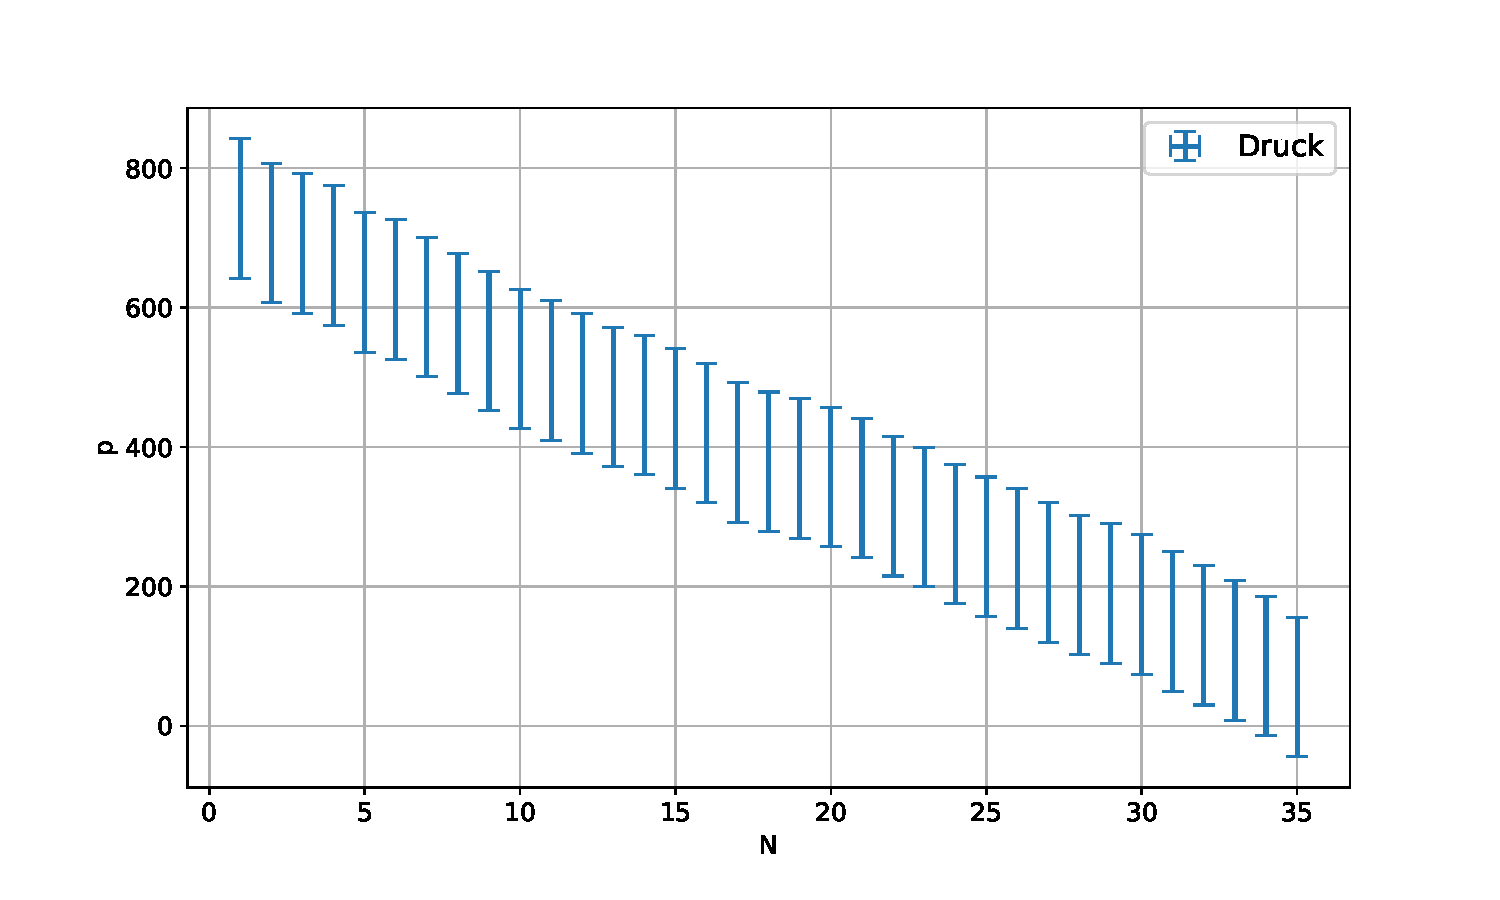
\includegraphics[width=0.9\textwidth]{images/CO2_Raus.pdf}
		\centering
		\caption{In der Küvette befindet sich CO$^2$. Der Druck wird kontinuierlich reduziert. Die gelbe Funktion ist ein linearer Fit.}
		\label{fig_co2_raus}
	\end{figure}
\begin{figure}[H]
		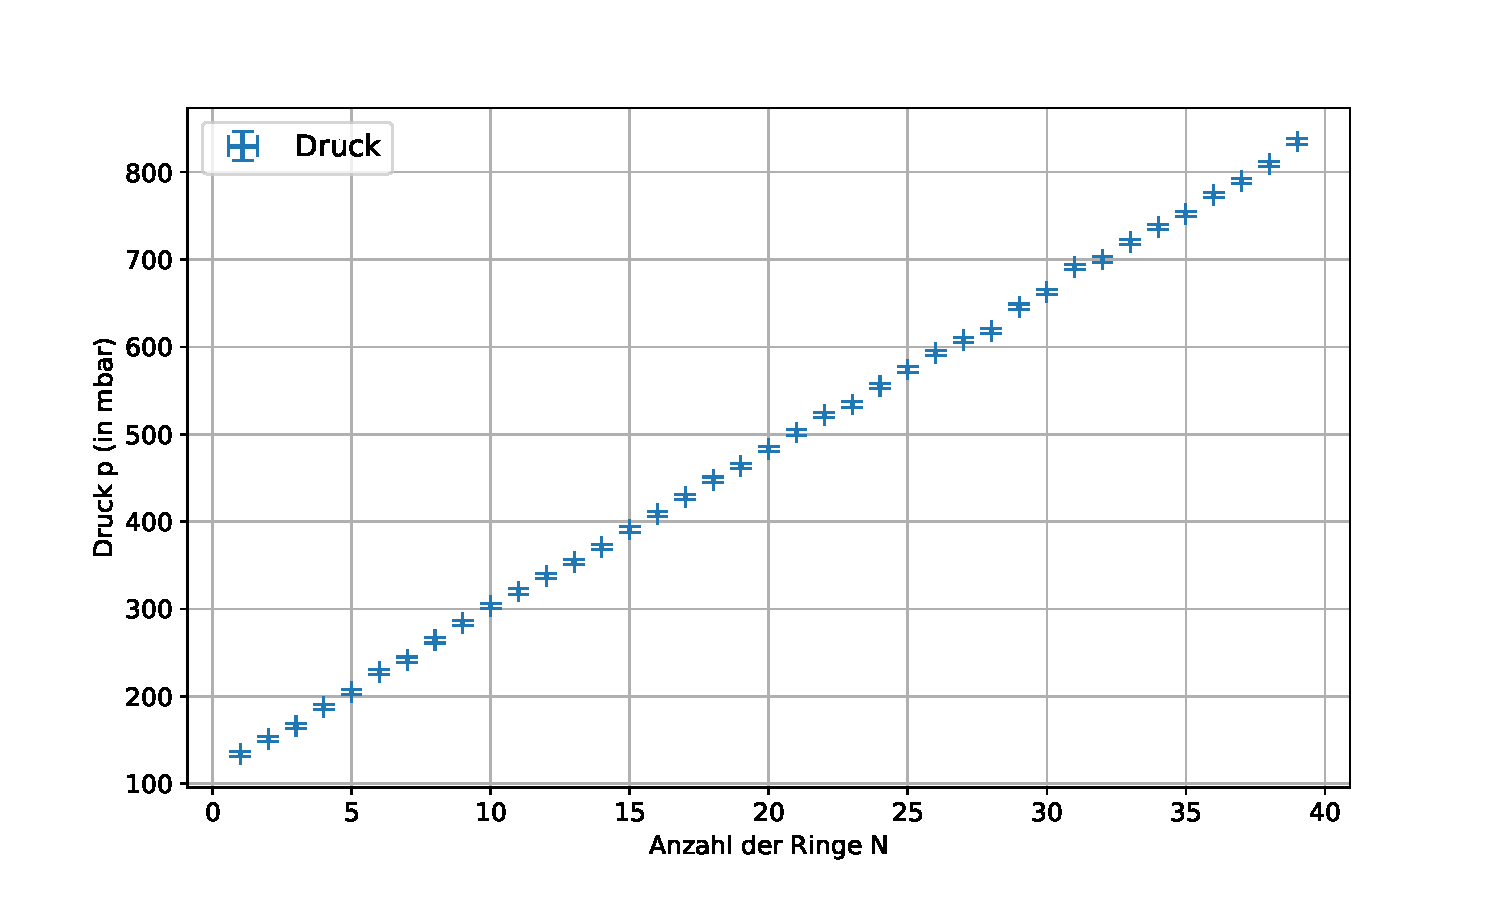
\includegraphics[width=0.9\textwidth]{images/CO2_Rein.pdf}
		\centering
		\caption{In der Küvette befindet sich CO$^2$. Der Druck wird kontinuierlich erhöht. Die gelbe Funktion ist ein linearer Fit.}
		\label{fig_co2_rein}
	\end{figure}

	In \cref{tb_gase} sind die aus den Fitparameter resultierenden Brechungsindizes der Gase aufgelistet.
	Dabei ist zu beachten, dass sich bei inverser Druckänderung auch die Interferenzringe in die umgekehrte Richtung verschieben.


	\begin{table}[H]
		\centering
		\begin{tabular}{| c | c | c |}
			\hline
			  Gas &  $\Delta p/\Delta m$ & $n(p=\SI{1013}{mbar})$\\ \hline
				Luft& \SI{28.81+-0.1}{mbar} & \SI{1.000327+-0.000029}{}\\
				&\SI{28.46+-0.11}{mbar}&\SI{1.000331+-0.000029}{}\\
				CO$^2$ & \SI{19.11+-0.18}{mbar} & \SI{1.000493+-0.000043}{}\\
				&\SI{18.28+-0.04}{mbar}&\SI{1.000514+-0.000045}{}\\
				\hline
		\end{tabular}
		\caption{}
		\label{tb_gase}
	\end{table}

	\subsubsection{Diskussion}
	% Bezug/Nutzen oder sonst was
	% auch hier die Hypothese wiederholen
	% keine Messwerte hier, nach manchen Menschen, zumindest "direkt" erstellte Diagramme net hier, auch wenn Lesbarkeit-bla
	%TODO siehe Kurzfassung

	%TODO geringe Schwankungen bei kontinuierlichem Messen sind ziemlich ahnbar
	%TODO rein ca. gleich wie raus erwartbar

	\section{Schlussfolgerung}
	% Rückgriff auf Hypothese und drittes Nennen dieser

	% Quellen zitieren, Websiten mit Zugriffsdatum
	% Verweise auf das Laborbuch (sind erlaubt)
	% Tabelle + Bilder mit Beschriftung
	\printbibliography
\end{document}
